\chapter{Methodology}\label{ch:methodology}
\section{Basic BTW Model Rules}

As mentioned in the Introduction, the BTW sandpile model is defined on a two-dimensional grid of a preset size with sand grains added at randomly chosen sites, prescribed toppling rules and open boundaries.

The first step of simulating a basic BTW sandpile model is to initialise an empty two-dimensional grid of preset size $N\times M$. At each step, one grain of sand is added to a randomly chosen grid point. After sand addition, if a grid point contains four or more grains of sand, four grains are removed from it, and one grain is added to each of its neighbours: the grid points above, below, left and right. If a neighbour of the toppling site lies outside the grid, the grain transferred in that direction is removed from the system. Toppling continues until every grid point contains fewer than four grains of sand. The state and avalanche properties are then recorded. Finally, the sand-addition and toppling process is repeated until the preset number of grain additions is reached.

\begin{figure}[htbp]
    \centering
    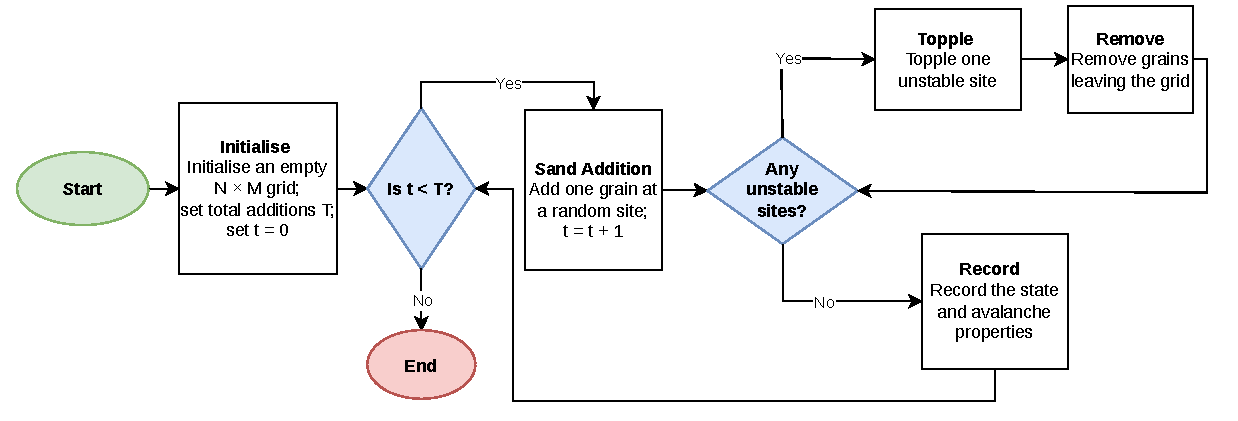
\includegraphics[width=0.9\linewidth]{figures/flowchart.pdf}
    \caption{Flowchart of the basic BTW sandpile simulation.}
    \label{fig:flowchart}
\end{figure}

Mathematically, we can consider the grid as an $N \times M$ matrix. Initially, all elements in the matrix are zero. When a grain of sand is added, the corresponding element in the matrix increases by one. 

Define $p_t(i,j)$ to denote the number of sand grains in row $i$, column $j$, at time t. If $p_t(i,j) \ge 4$, the following updates are applied:
\[
\begin{aligned}
p_t(i,j) &= p_t(i,j)-4,\\
p_t(i\pm1,j) &= p_t(i\pm1,j)+1,\\
p_t(i,j\pm1) &= p_t(i,j\pm1)+1.
\end{aligned}
\]
For example:
\[
\begin{pmatrix}
0 & 3 & 1 \\
1 & 3 & 0 \\
0 & 0 & 0
\end{pmatrix}
\;\rightarrow\;
\begin{pmatrix}
0 & 3 & 1 \\
1 & 4 & 0 \\
0 & 0 & 0
\end{pmatrix}
\;\rightarrow\;
\begin{pmatrix}
0 & 4 & 1 \\
2 & 0 & 1 \\
0 & 1 & 0
\end{pmatrix}
\;\rightarrow\;
\begin{pmatrix}
1 & 0 & 2 \\
2 & 1 & 1 \\
0 & 1 & 0
\end{pmatrix}
\]

First, one grain of sand is added to position $(2,2)$. This grid point now contains four grains of sand, so toppling occurs. Four grains of sand are removed from position $(2,2)$, and the number of grains at each of its neighbours, positions $(1,2)$, $(2,1)$, $(3,2)$ and $(2,3)$, increases by one. Now, position $(1,2)$ contains four grains of sand, so toppling happens again. Since one of the neighbours of position $(1,2)$ is outside the matrix, one grain of sand is lost from the system.

\newpage

It is important for the table to have finite open boundaries. These allow sand to leave the system, preventing the total number of sand grains from increasing indefinitely. If we have an infinite lattice but drop sand only on a finite subset of the lattice, sites outside may also topple and transfer sand back into it. Therefore, the subset cannot be treated as a finite system with open boundaries.

\section{Measured Properties}

In this project, I will record and analyse the following avalanche properties:

\begin{description}
	\item[Topples] The total number of toppling events during an avalanche.
	\item[Area] The number of distinct sites that topple during an avalanche.
	\item[Loss] The number of sand grains lost through the open boundaries during an avalanche.
	\item[Length] The maximum Manhattan distance from the initial toppling site to any site toppled in the avalanche.
\end{description}

The avalanche length measures how far the toppling activity spreads from the initial toppling site. Manhattan distance, calculated as $|x_1-x_2| + |y_1-y_2|$ between sites $(x_1,y_1)$ and $(x_2,y_2)$, is used because sand is transferred only to the neighbours above, below, left and right.

Another important property that will be focused on is the average height of the pile. For an $N \times M$ grid, its average height is calculated as:
$$\langle p_t \rangle := \frac{1}{NM}\sum_{i,j}p_t(i,j) $$

\section{Simulation Setup}

To simulate the BTW model using Python, I initialise each pile as a $50 \times 50$ matrix with all elements set to zero. A total of $100{,}000$ grains of sand are added to each pile, one at a time. I independently simulate five piles to assess the variability between runs. To ensure the reproducibility of the random selection, I set the seed to 1643210. 

I first define a sand addition function that takes a matrix as input, then randomly selects one element from it and increments its value by 1. 

The toppling rule is implemented by taking a matrix as input and using a while loop that continues until no element in the matrix has a value greater than or equal to 4. Inside the while loop, when a position with a value greater than or equal to 4 is found, its value is decreased by 4. For each neighbour, an if statement checks whether it lies within the matrix. If it is, its value is increased by one. Otherwise, the loss count is increased by one. The function records the row and column indices of all toppling events, the total loss, and the final matrix after all toppling activity has ceased. Additionally, I define three functions to calculate topples, area, and length using the output from the toppling function. If no toppling occurs after a grain addition, all four avalanche properties are recorded as zero.

For each pile, the sand-addition and toppling functions are called repeatedly 100,000 times. After each grain addition and toppling, the four avalanche properties and the average height are recorded. Then I generate a plot of the average pile height against the number of grains added. Since all piles are initially empty, they require a number of grain additions to reach a steady state. The plot is used to identify when the average pile height begins to fluctuate around a stable level. Based on this observation, the first 10,000 records from each pile are removed, and the remaining records are used for further analysis of the avalanche properties. Using these remaining records, I generate linear-scale, semi-log, and log-log plots for Topples, Area, Loss, and Length to explore their distribution shapes and identify candidate distributions for fitting. I also plot heat maps of the final configurations to compare the spatial distributions of sand heights in the basic and extended models.

\subsection{Statistical Analysis}
\subsubsection{Topples}

For the Topples property, I attempt to fit a power law. In particular, I first exclude zero values since $\log(0)$ is undefined. Let $x$ denote a positive number of topples and $y$ be its corresponding observed frequency. The power-law relationship can be written as
$$y = Ax^\alpha,$$
and taking logarithms gives

$$\log(y) = \log(A) + \alpha \log(x).$$

Therefore, I use \texttt{np.polyfit} to perform a fit of $\log(y)$ against $\log(x)$ and estimate $A$ and $\alpha$. Then I plot the fitted curve and the observed frequencies on the same log-log plot. This estimation is performed separately for each pile.

Mean Absolute Error (MAE) and Root Mean Square Error (RMSE) are used to evaluate the differences between the observed and fitted frequencies:
\begin{align*}
	\text{MAE} &= \frac{1}{n}\sum_{i=1}^{n}|y_i-\hat{y}_i|, \\[6pt]
	\text{RMSE} &= \sqrt{\frac{1}{n}\sum_{i=1}^{n}(y_i-\hat{y}_i)^2}.
\end{align*}
where $n$ is the number of distinct positive Topples values observed, $y_i$ and $\hat{y}_i$ are the observed and fitted frequencies at each value, respectively. Both errors are calculated on the original frequency scale.

\subsubsection{Area}
Similarly, for the Area property, I first fit a power law, but the fitted curve does not describe the observed frequency distribution well. Therefore, I further check if the distribution can be expressed as a log-normal distribution. 

The log-normal distribution can be expressed as:

$$\log(X) \sim N(\mu, \sigma^2)$$
where $X$ represents Area. I first estimate $\mu$ and $\sigma^2$ from the logarithms of the positive Area values by 
\begin{align*}
	N &= \sum_{i} y_i,\\[6pt]
	\hat\mu&= \frac{\sum_{i}(y_i * \log(x_i))}{N}, \\[6pt]
	\hat\sigma^2 &= \frac{\sum_{i}\{y_i *[\log(x_i)-\hat\mu]^2\}}{N}.
\end{align*}

 Since the log-normal distribution is continuous, I approximate the frequency at each integer area value using the probability within a centred unit-width interval. The fitted frequency is calculated as

$$\hat{y} = N[P(X \le x+0.5)- P(X\le x-0.5)].$$ 

Similarly, the fitted frequencies are compared with the observed Area frequencies on the same log-log plot and are used to calculate MAE and RMSE.
\subsubsection{Loss}
For the Loss property, I first fit a geometric distribution that includes zero, with probability mass function:
$$\Pr(X=x) = p(1-p)^x, \qquad x=0,1,2,\ldots,$$
where $X$ represents Loss. Since the mean is $\mu = \frac{1-p}{p}$, I estimate $p$ using the sample mean $\bar{x}$:
$$\hat p = \frac{1}{\bar{x}+1}.$$
The fitted frequencies are then calculated as:
\begin{align*}
	N &= \sum_i y_i, \\[6pt]
	\hat y &= N\hat p(1-\hat p)^x.
\end{align*}
Since the fitted curve does not describe the observed frequencies well on the semi-log plot, I then fit a geometric distribution to the positive Loss values, excluding zero.

For a geometric distribution that excludes zero, the probability mass function becomes:
$$\Pr(X=x) = p(1-p)^{x-1}$$

The mean is now $\mu = \frac{1}{p}$, so $\hat p = \frac{1}{\bar{x}}$, where $\bar{x}$ is calculated from the positive Loss values. I calculate the fitted frequencies using the updated probability mass function and the number of positive observations, and plot the fitted curve and the observed frequencies on the same semi-log plot. MAE and RMSE are also calculated and recorded. 

I also try to fit a log-normal distribution, plot the fitted curve and calculate MAE and RMSE to compare the two distributions.

\subsubsection{Length}

For the Length property, I also fit a log-normal distribution to the observed frequencies. I use the same fitting and error calculation procedures as for the log-normal fit to Area and Loss.

\subsubsection{Correlation}
In order to explore the correlations between the four properties, I first create pairwise scatter plots using only data from the first pile, where the x-axis represents one property and the y-axis represents another. For each pile, I calculate the Spearman correlations between the properties and present them in a correlation matrix. 

I choose Spearman correlation because it measures monotonic relationships between properties without requiring these relationships to be linear. It is calculated using the ranks of the observations.

